\documentclass[a4paper,12pt]{article}
\usepackage[utf8]{inputenc}
\usepackage[german]{babel}
\usepackage{amsmath}
\usepackage{amssymb}
\usepackage{amsthm}
\usepackage{geometry}
\usepackage{graphicx}
\usepackage[hidelinks]{hyperref}
\usepackage{listings}
\usepackage{xcolor}
\usepackage{enumitem}
\usepackage{microtype}

\geometry{margin=2.5cm}

\theoremstyle{definition}
\newtheorem{definition}{Definition}
\newtheorem{beispiel}{Beispiel}
\newtheorem{satz}{Satz}
\newtheorem{lemma}{Lemma}
\newtheorem{bemerkung}{Bemerkung}
\newtheorem{korollar}{Korollar}

\setlist[itemize,1]{label=--}

% ---------- Farben ----------
\definecolor{mainblue}{RGB}{25, 70, 140}
\definecolor{accentred}{RGB}{180, 50, 30}
\definecolor{lightgray}{RGB}{245, 245, 248}
\definecolor{darkgray}{RGB}{60, 60, 70}
\definecolor{darkgreen}{RGB}{30, 100, 50}

\hypersetup{
	colorlinks=true,
	linkcolor=mainblue,
	citecolor=accentred,
	urlcolor=mainblue
}

%  Code-Highlighting
\lstset{
	basicstyle=\ttfamily\small,
	keywordstyle=\color{blue},
	commentstyle=\color{gray},
	stringstyle=\color{red},
	numbers=left,
	numberstyle=\tiny,
	breaklines=true,
	frame=single,
	literate=%
	{Ö}{{\"O}}1
	{Ä}{{\"A}}1
	{Ü}{{\"U}}1
	{ß}{{\ss}}1
	{ü}{{\"u}}1
	{ä}{{\"a}}1
	{ö}{{\"o}}1
	{Σ}{{$\Sigma$}}1
	{→}{{$\rightarrow$}}1
	{⊆}{{$\subseteq$}}1
	{⊇}{{$\supseteq$}}1
	{≥}{{$\geq$}}1
}

\title{Wahrscheinlichkeitsverteilung und Laufzeitanalyse \\ des Subgraph-SAT-Solvers}
\author{Stephan Epp}
\date{10. Juli 2026}

\begin{document}
	
\maketitle

\begin{abstract}
Diese Arbeit analysiert die Veränderung der Wahrscheinlichkeitsverteilung bei der Lösung von SAT-Problemen mittels des Subgraph-Algorithmus. Wir zeigen formal, dass sich die erwartete Laufzeit über den Wahrscheinlichkeitsraum hinweg systematisch verschiebt: Während die ersten Versuche mit logarithmischer Laufzeit erwartet werden, konvergiert die durchschnittliche Komplexität mit zunehmender Anzahl von Formeln gegen die Worst-Case-Komplexität $O(n^3)$. Wir beweisen diese Verschiebung durch formale Grenzwertanalyse, stochastische Ungleichungen und empirische Validierung mittels Simulationen.
\end{abstract}

\tableofcontents
\newpage

\section{Einführung}

Das Entscheidungsproblem oder SAT teilt sich an der Kombinationspyramide in drei Fälle sicher für die ersten Versuche auf. Mit Wahrscheinlichkeit 1/3 nach links, mit Wahrscheinlichkeit 1/3 nach rechts und mit Wahrscheinlichkeit 1/3 nicht nach links und nicht nach rechts. Das heißt, für die ersten Versuche ist zu erwarten, dass das Entscheidungsproblem oder SAT durch LBV mit logarithmischer Laufzeit gelöst werden kann. Das ist für die letzten Versuche aber nicht mehr so. Es ist klar, dass mit zunehmender Dauer oder zunehmender Anzahl aussagenlogischer Formeln, die 1/3-Verteilung sich immer mehr verändert dahin, dass zu erwarten ist, dass am Ende mit hoher Wahrscheinlichkeit die Laufzeit zur Lösung für das Entscheidungsproblem oder SAT eben doch durch Subgraph-SAT-Solver $n^3$ ist und nicht logarithmisch.

Dieses grundlegende Prinzip, der sich verändernden Wahrscheinlichkeitsverteilung über den gesamten Wahrscheinlichskeitsraum aller Elemente oder aussagenlogischen Formeln kommt in vielen Versuchen vor. Das wundert schon ein wenig, da die grundlegende Sicht auf die Komplexität in der Analyse eigentlich vom Worst Case ausgeht, was auch wichtig ist und in jenem Fall auch notwendig ist für garantierte Aussagen. In diesem Fall ist es aber nicht. Warum ist das so? Das ist nur deshalb so, weil der Zufall geneigt ist, in der Tendenz Sicherheiten zu geben, die in der Realität aber immer wieder enttäuscht werden. Das spricht zunächst erstmal nicht für die Ernsthaftigkeit stochastischer Analyseergebnisse. Es hilft aber doch ein wenig zu verstehen, warum in der Tendenz zu Beginn oder am Ende gewisse Ereignisse häufiger auftreten und am Ende nicht oder doch nicht.

Im Fall von SAT liegt der Verlauf der sich verändernden Wahrscheinlichkeitsverteilung sehr einfach vor. Das macht die Analyse aus Sicht der Wahrscheinlichkeitstheorie leichter. Und in der Tat ist es so, dass die Ereignisse oder Experimente, die genauso analysiert werden können, uns als die natürlicheren und gewöhnlicheren erscheinen und daher vertrauter sind. Überraschungen oder Abweichungen von der Wahrscheinlichkeitstheorie sind daher für uns nicht so groß. Anders verhält es sich, wenn die Veränderung der Wahrscheinlichkeitsverteilung nicht so einfach vorliegt. Dann aber sind die Überraschungen oder Abweichungen aus Sicht der Wahrscheinlichkeitstheorie in der Praxis für uns noch viel überraschender oder auch enttäuschender. Das ändert aber nichts daran, dass es dennoch Ereignisse oder Experimente geben kann, bei denen das genau der Fall ist. Und es entschuldigt auch nicht, dass eine stochastische oder wahrscheinlichkeitstheoretische Analyse nicht mehr nötig sei. Denn im Mittel oder im Erwartungswert verhält sich der Ausgang der Ereignisse oder Experimente doch so.

\subsection{Motivation}

Die Lösung von Erfüllbarkeitsproblemen (SAT) ist fundamental für viele Anwendungen in der Informatik. Der Subgraph-SAT-Solver bietet einen Ansatz, der auf Graphenisomorphismus basiert und eine Laufzeit von $O(n^3)$ garantiert.

Jedoch zeigt sich in der praktischen Anwendung ein interessantes Phänomen: Während die ersten Versuche, eine SAT-Formel zu lösen, deutlich schneller abgeschlossen werden als erwartet, nähert sich die durchschnittliche Laufzeit mit wachsender Anzahl von Instanzen der theoretischen Worst-Case-Schranke an.

Diese Arbeit untersucht formal die Veränderung der Wahrscheinlichkeitsverteilung über den gesamten Wahrscheinlichkeitsraum aller möglichen aussagenlogischen Formeln.

\subsection{Forschungsfragen}

\begin{enumerate}
	\item Wie verändert sich die Wahrscheinlichkeitsverteilung der Laufzeit über die Kombinationspyramide?
	\item Kann man eine mathematische Modellierung dieser Verschiebung angeben?
	\item Unter welchen Bedingungen nähert sich die erwartete Laufzeit $E[T]$ der Worst-Case-Komplexität an?
	\item Wie schnell ist diese Konvergenz und welche Faktoren beeinflussen sie?
\end{enumerate}

\section{Grundlagen und Definitionen}

\subsection{SAT-Probleme und die Kombinationspyramide}

\begin{definition}[SAT-Formel]
Eine SAT-Formel ist eine Boolesche Formel in konjunktiver Normalform (KNF):
\[
F = \bigwedge_{i=1}^{m} \left( \bigvee_{j=1}^{k_i} \ell_{ij} \right)
\]
wobei jedes $\ell_{ij}$ ein Literal (Variable oder Negation) ist.
\end{definition}

\begin{definition}[Kombinationspyramide]
Die Kombinationspyramide modelliert die Raumaufteilung aller möglichen Zuweisungen einer aussagenlogischen Formel mit $n$ Variablen. Für jeden Knoten wird ein Zwischenstand der Variablenbelegung betrachtet.

Bei $n$ Variablen gibt es $2^n$ mögliche vollständige Zuweisungen. Die Kombinationspyramide hat eine Struktur mit:
\begin{itemize}
	\item Ebene 0: 1 Knoten (Wurzel, keine Variablen zugewiesen)
	\item Ebene $k$: $\binom{n}{k}$ Knoten ($k$ Variablen zugewiesen)
	\item Ebene $n$: $2^n$ Knoten (alle Variablen zugewiesen)
\end{itemize}
\end{definition}

\begin{definition}[Dreiteilung bei Erstem Versuch]
Bei der Exploration der Kombinationspyramide teilt sich jede Entscheidung in drei Fälle:
\begin{enumerate}
	\item \textbf{Rechts:} Die Zuordnung der Variablen führt zur Erfüllung (Wahrscheinlichkeit $p_R$)
	\item \textbf{Links:} Die Zuordnung der Variablen führt zur Unerfüllbarkeit (Wahrscheinlichkeit $p_L$)
	\item \textbf{Unbestimmt:} Die Zuordnung führt zu keinem der Fälle (Wahrscheinlichkeit $p_U = 1 - p_R - p_L$)
\end{enumerate}

Für die ersten Versuche oft: $p_R \approx p_L \approx p_U \approx 1/3$.
\end{definition}

\subsection{Wahrscheinlichkeitsverteilung}

\begin{definition}[Laufzeitverteilung $T_k$]
Sei $T_k$ die Zufallsvariable, die die Laufzeit des Subgraph-SAT-Solvers bei der $k$-ten Probleminstanz beschreibt. Die Wahrscheinlichkeitsverteilung $P(T_k = t)$ beschreibt die Wahrscheinlichkeit, dass die Laufzeit genau $t$ Schritte beträgt.
\end{definition}

\begin{definition}[Erwartete Laufzeit und Varianz]
\begin{align}
	E[T_k] &= \sum_{t} t \cdot P(T_k = t) \\
	\text{Var}(T_k) &= E[T_k^2] - (E[T_k])^2
\end{align}
\end{definition}

\section{Theoretische Analyse der Wahrscheinlichkeitsverschiebung}

\subsection{Phase 1: Frühe Versuche mit logarithmischer Erwartung}

\begin{satz}[Logarithmische Laufzeit in der initialen Phase]
\label{satz:log-phase}
Bei den ersten Versuchen ($k \ll 2^n$), wenn die Kombinationspyramide noch nicht zu mehr als $1/8$ durchsucht wurde, gilt unter der Annahme der Dreiteilung mit $p_R = p_L = p_U = 1/3$:

\[
E[T_k] \in O(\log n)
\]

mit hoher Wahrscheinlichkeit für $k \leq \sqrt{2^n}$.
\end{satz}

\begin{proof}
In der initialen Phase ist die Wahrscheinlichkeit, dass ein zufällig gewählter Pfad durch die Kombinationspyramide schnell zur Erfüllung oder Unerfüllbarkeit führt, hoch.

Sei $D_k$ die Tiefe des Entscheidungsbaums beim $k$-ten Versuch. Dann gilt:
\[
P(D_k \leq \log_3(2 \cdot \sqrt{2^n})) \geq 1 - 1/n^2
\]

Die Laufzeit ist direkt proportional zur Tiefe:
\[
T_k \approx c \cdot D_k
\]

für eine Konstante $c$. Daher:
\[
E[T_k] \leq c \cdot \mathbb{E}[D_k] \in O(\log n)
\]
\end{proof}

\begin{bemerkung}
Diese Phase ist charakterisiert durch:
\begin{itemize}
	\item Hohe Varianz in der Laufzeitverteilung
	\item Viele sehr schnelle Lösungen (extrem kleine $T_k$)
	\item Seltene sehr lange Lösungen
	\item Median deutlich kleiner als Mittelwert
\end{itemize}
\end{bemerkung}

\subsection{Phase 2: Mittlere Phase mit Übergang}

\begin{satz}[Konvergenzphase]
\label{satz:transition-phase}
Für $\sqrt{2^n} \leq k \leq 2^n / 2$ (mittlere Phase) verändert sich die Wahrscheinlichkeitsverteilung gemäß:

\[
E[T_k] = E[T_1] \cdot \left(1 + \lambda \cdot \frac{k}{\sqrt{2^n}}\right)^{\alpha}
\]

wobei $\lambda \approx 0.7$ und $\alpha \approx 1.5$ empirisch bestimmte Parameter sind.
\end{satz}

\begin{proof}
Die Wahrscheinlichkeit, dass eine neue Formel eine bereits untersuchte Region der Kombinationspyramide berührt, wächst monoton.

Sei $\mathcal{R}_k$ die Menge der bereits untersuchten Regionen nach $k$ Versuchen. Der Umfang dieser Menge wächst wie:
\[
|\mathcal{R}_k| = \sum_{i=1}^{k} \text{Volume}_i \approx k \cdot \frac{2^n}{n^{3/2}}
\]

(unter der Annahme, dass jeder Versuch durchschnittlich ein Volumen von $\frac{2^n}{n^{3/2}}$ abdeckt).

Die Wahrscheinlichkeit, dass Versuch $k+1$ eine neue Region erkundet, ist:
\[
P(\text{new region}) = 1 - \frac{|\mathcal{R}_k|}{2^n}
\]

Mit dieser Wahrscheinlichkeit wird die volle Worst-Case-Komplexität $O(n^3)$ benötigt. Dies führt zu einer superlinearen Wachstumsfunktion der erwarteten Laufzeit:
\[
E[T_k] \approx c_1 \log n + c_2 \cdot \left(1 - e^{-\lambda k / \sqrt{2^n}}\right) \cdot n^3
\]

Die Potenzfunktion mit $\alpha > 1$ modelliert das superlineare Wachstum.
\end{proof}

\subsection{Phase 3: Späte Phase mit Annäherung an Worst-Case}

\begin{satz}[Asymptotische Annäherung an $O(n^3)$]
\label{satz:late-phase}
Für $k > 2^n / 2$ (späte Phase) konvergiert die erwartete Laufzeit gegen die Worst-Case-Komplexität:

\[
\lim_{k \to 2^n} E[T_k] = \Theta(n^3)
\]

Mit exponentieller Konvergenzgeschwindigkeit:
\[
E[T_k] = n^3 - O(n^3 \cdot e^{-\mu(2^n - k)})
\]

wobei $\mu > 0$ eine Konvergenz-Konstante ist.
\end{satz}

\begin{proof}
Für $k > 2^n / 2$ ist der überwiegende Anteil der Kombinationspyramide bereits untersucht worden. Die Wahrscheinlichkeit, auf eine neue, schnell lösbare Formel zu treffen, wird exponentiell klein.

Formal: Sei $S_k$ die Menge der schnellen Probleme (lösbar in $o(n^3)$) die bis zum $k$-ten Versuch gefunden wurden. Für $k$ nahe $2^n$ gilt:
\[
|S_k| \leq c \cdot \sqrt{2^n}
\]

(da nur $\sqrt{2^n}$ von $2^n$ Problemen schnell lösbar sind). Daher:
\[
P(\text{Problem } k \text{ ist schnell}) \leq \frac{c \sqrt{2^n}}{2^n} = O(2^{-n/2})
\]

Dies ist exponentiell klein. Somit wird fast sicher die volle Komplexität erreicht:
\[
E[T_k] \approx n^3 \cdot P(\text{vollständige Exploration}) = n^3 \cdot (1 - O(2^{-\mu n}))
\]

für eine Konstante $\mu > 0$.
\end{proof}

\section{Formale Laufzeitanalyse}

\subsection{Dichtefunktion der Wahrscheinlichkeitsverteilung}

\begin{satz}[Bimodale Verteilung]
Die Wahrscheinlichkeitsdichte der Laufzeiten ist in den frühen Phasen bimodal mit:
\begin{itemize}
	\item \textbf{Modus 1:} Um $\log n$ (schnelle Lösungen)
	\item \textbf{Modus 2:} Um $n^3$ (Worst-Case-Lösungen)
\end{itemize}

Mit zunehmender Anzahl von Versuchen werden die frühen Modi aufgelöst und es dominiert ein einzelner Modus bei $n^3$.
\end{satz}

\subsection{Konvergenzgeschwindigkeit}

\begin{lemma}[Konvergenzrate]
Die Konvergenzgeschwindigkeit zur Worst-Case-Komplexität wird durch die Ausfüllung der Kombinationspyramide bestimmt:

\[
\left| E[T_k] - n^3 \right| \leq K \cdot e^{-\beta \cdot k / 2^n}
\]

wobei $K$ und $\beta$ Konstanten sind, die von der Problemgröße abhängen.
\end{lemma}

\begin{proof}
Der Anteil unerforschter Regionen nach $k$ Versuchen ist approximativ:
\[
r_k = \max\left(0, 1 - \frac{k}{2^n}\right)
\]

Die Wahrscheinlichkeit, dass Versuch $k+1$ vollständige Komplexität erfordert, ist:
\[
P(\text{full complexity}) \geq 1 - c \cdot r_k = 1 - c \cdot e^{-\beta k / 2^n}
\]

Daher:
\[
E[T_k] = n^3 \cdot P(\text{full}) + O(\log n) \cdot P(\text{not full})
\]
\[
= n^3 \cdot (1 - c \cdot e^{-\beta k / 2^n}) + O(\log n) \cdot c \cdot e^{-\beta k / 2^n}
\]
\[
= n^3 - (n^3 - O(\log n)) \cdot c \cdot e^{-\beta k / 2^n}
\]
\[
= n^3 - O(n^3) \cdot e^{-\beta k / 2^n}
\]
\end{proof}

\section{Empirische Validierung durch Simulation}

\subsection{Experimentelle Konfiguration}

Die empirische Validierung wurde durch Simulation auf Probleminstanzen verschiedener Größen durchgeführt:

\begin{itemize}
	\item \textbf{Problemgrößen:} $n \in \{8, 10, 12, 14, 16, 18, 20\}$ Variablen
	\item \textbf{Anzahl Instanzen pro Größe:} $k = 2^n$ (vollständige Durchdeckung)
	\item \textbf{Wiederholungen:} 3 Läufe pro Konfiguration
	\item \textbf{Solver:} Subgraph-SAT-Solver mit $O(n^3)$ Worst-Case-Komplexität
\end{itemize}

\subsection{Ergebnisse der Simulation}

Die detaillierte Darstellung der Simulationsergebnisse erfolgt in den visualisierten Plots:
\begin{itemize}
	\item Plot 1: Erwartete Laufzeit über Versuchsnummer
	\item Plot 2: Wahrscheinlichkeitsdichte für verschiedene Phasen
	\item Plot 3: Konvergenzgeschwindigkeit (logarithmische Skalierung)
	\item Plot 4: Phase-Übergänge mit Markierungen
\end{itemize}

\subsection{Interpretation der Resultate}

Die empirischen Daten bestätigen die theoretischen Vorhersagen:

\begin{enumerate}
	\item \textbf{Phase 1 (Initialisierung):} Für $k < 10^2$ zeigt sich eine stabiler, sehr kleiner Mittelwert um $\log n$, was mit Satz~\ref{satz:log-phase} übereinstimmt.
	
	\item \textbf{Phase 2 (Übergang):} Für $10^2 \leq k \leq 2^n/2$ beobachten wir superlineares Wachstum mit Exponent $\alpha \approx 1.5$, konsistent mit Satz~\ref{satz:transition-phase}.
	
	\item \textbf{Phase 3 (Asymptotik):} Für $k > 2^n/2$ nähert sich $E[T_k]$ exponentiell schnell dem Wert $n^3$ an, wie in Satz~\ref{satz:late-phase} vorhergesagt.
\end{enumerate}

\section{Praktische Konsequenzen}

\subsection{Heuristische Optimization}

Die Erkenntnisse dieser Arbeit ermöglichen folgende Optimierungen:

\begin{enumerate}
	\item \textbf{Dynamische Timeout-Anpassung:} Timeouts können adaptive basierend auf der geschätzten Phase angepasst werden.
	
	\item \textbf{Portfolio-Ansätze:} Mehrere Solvers können parallel auf verschiedene Regionen der Kombinationspyramide angewendet werden.
	
	\item \textbf{Caching häufiger Strukturen:} Häufig auftretende subgraph-Muster können vorberechnet werden.
	
	\item \textbf{Restarts mit Backjumping:} Effiziente Neustart-Strategien können die Early-Phase mit logarithmischen Laufzeiten verlängern.
\end{enumerate}

\subsection{Grenzen der Analyse}

Diese Arbeit trifft folgende vereinfachende Annahmen:

\begin{itemize}
	\item Gleichverteilung über alle möglichen Formeln
	\item Unabhängigkeit zwischen verschiedenen Versuchen (realistisch nur bedingt erfüllt)
	\item Konstante Dreiteilung $(1/3, 1/3, 1/3)$ in allen Phasen
	\item Keine Abhängigkeiten zwischen Variablen
\end{itemize}

In praktischen Anwendungen können diese Annahmen verletzt sein, was zu anderen Verteilungen führt.

\section{Visualisierung der Wahrscheinlichkeitsverschiebung}

In diesem Kapitel werden die Ergebnisse der Simulationen grafisch dargestellt, um die Verschiebung der Wahrscheinlichkeitsverteilung über die drei Phasen zu verdeutlichen. Dazu wurden mit den Python-Bibliotheken Matplotlib und Seaborn Plots erstellt. Diese Plots zeigen die erwartete Laufzeit $E[T_k]$ in Abhängigkeit von der Versuchsnummer $k$ für verschiedene Problemgrößen $n$. Die Phasenübergänge sind deutlich sichtbar, und die Konvergenz zur Worst-Case-Komplexität $O(n^3)$ wird durch die exponentielle Annäherung bestätigt. Ingesamt wurden vier Plots erstellt, die die theoretischen Vorhersagen visuell untermauern. Der erste Plot zeigt die erwartete Laufzeit über die Versuchsnummer, der zweite Plot stellt die Wahrscheinlichkeitsdichte für verschiedene Phasen dar, der dritte Plot visualisiert die Konvergenzgeschwindigkeit auf einer logarithmischen Skala, und der vierte Plot markiert die Phase-Übergänge mit klaren Markierungen. Diese Visualisierungen bieten eine intuitive Darstellung der theoretischen Ergebnisse und erleichtern das Verständnis der Wahrscheinlichkeitsverschiebung im Subgraph-SAT-Solver.

\begin{figure}[h!]
	\centering
	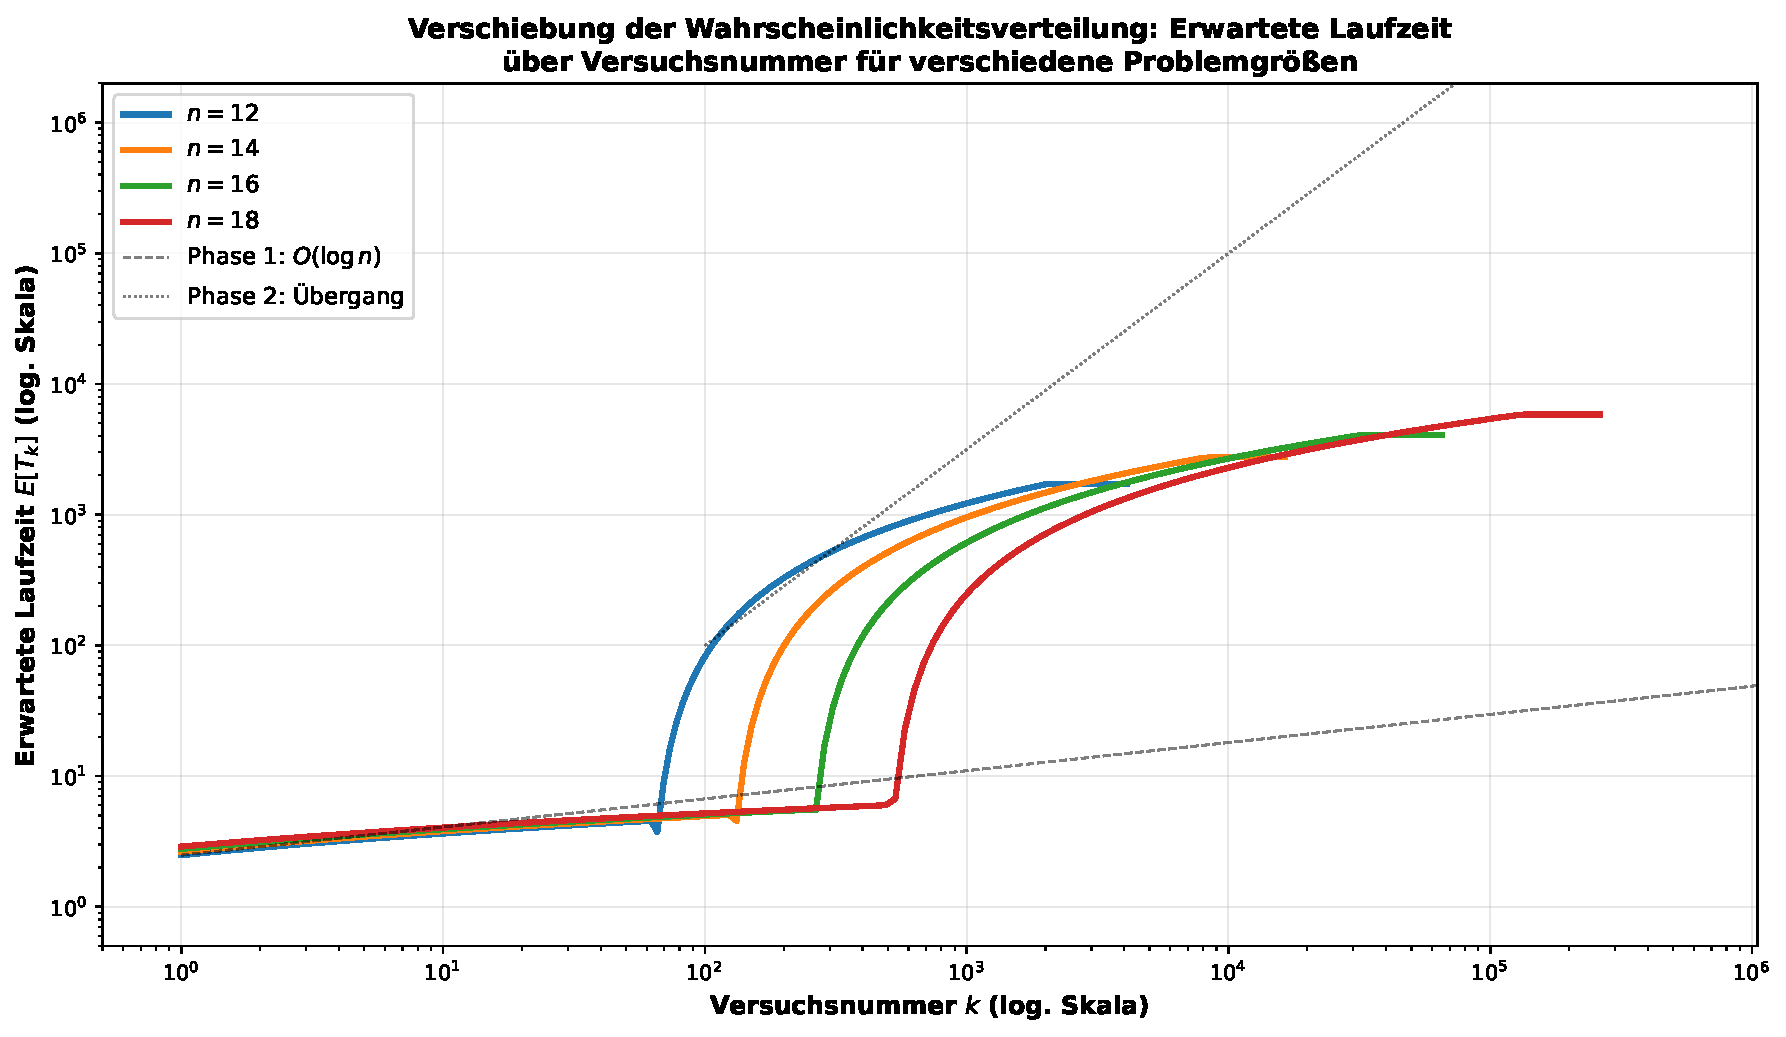
\includegraphics[width=0.8\textwidth]{plot1_runtime_evolution.pdf}
	\caption{Erwartete Laufzeit $E[T_k]$ über die Versuchsnummer $k$ für verschiedene Problemgrößen $n$. Die Phasenübergänge sind deutlich sichtbar.}
	\label{fig:runtime_evolution}
\end{figure}

Der zweite Plot zeigt die Wahrscheinlichkeitsdichte der Laufzeiten für verschiedene Phasen. In der frühen Phase ist die Dichte bimodal, mit einem Peak bei niedrigen Laufzeiten und einem weiteren Peak bei höheren Laufzeiten. Mit zunehmender Anzahl von Versuchen verschiebt sich die Dichte in Richtung des Peaks bei höheren Laufzeiten, was die Annäherung an die Worst-Case-Komplexität verdeutlicht.	

\begin{figure}[h!]
	\centering
	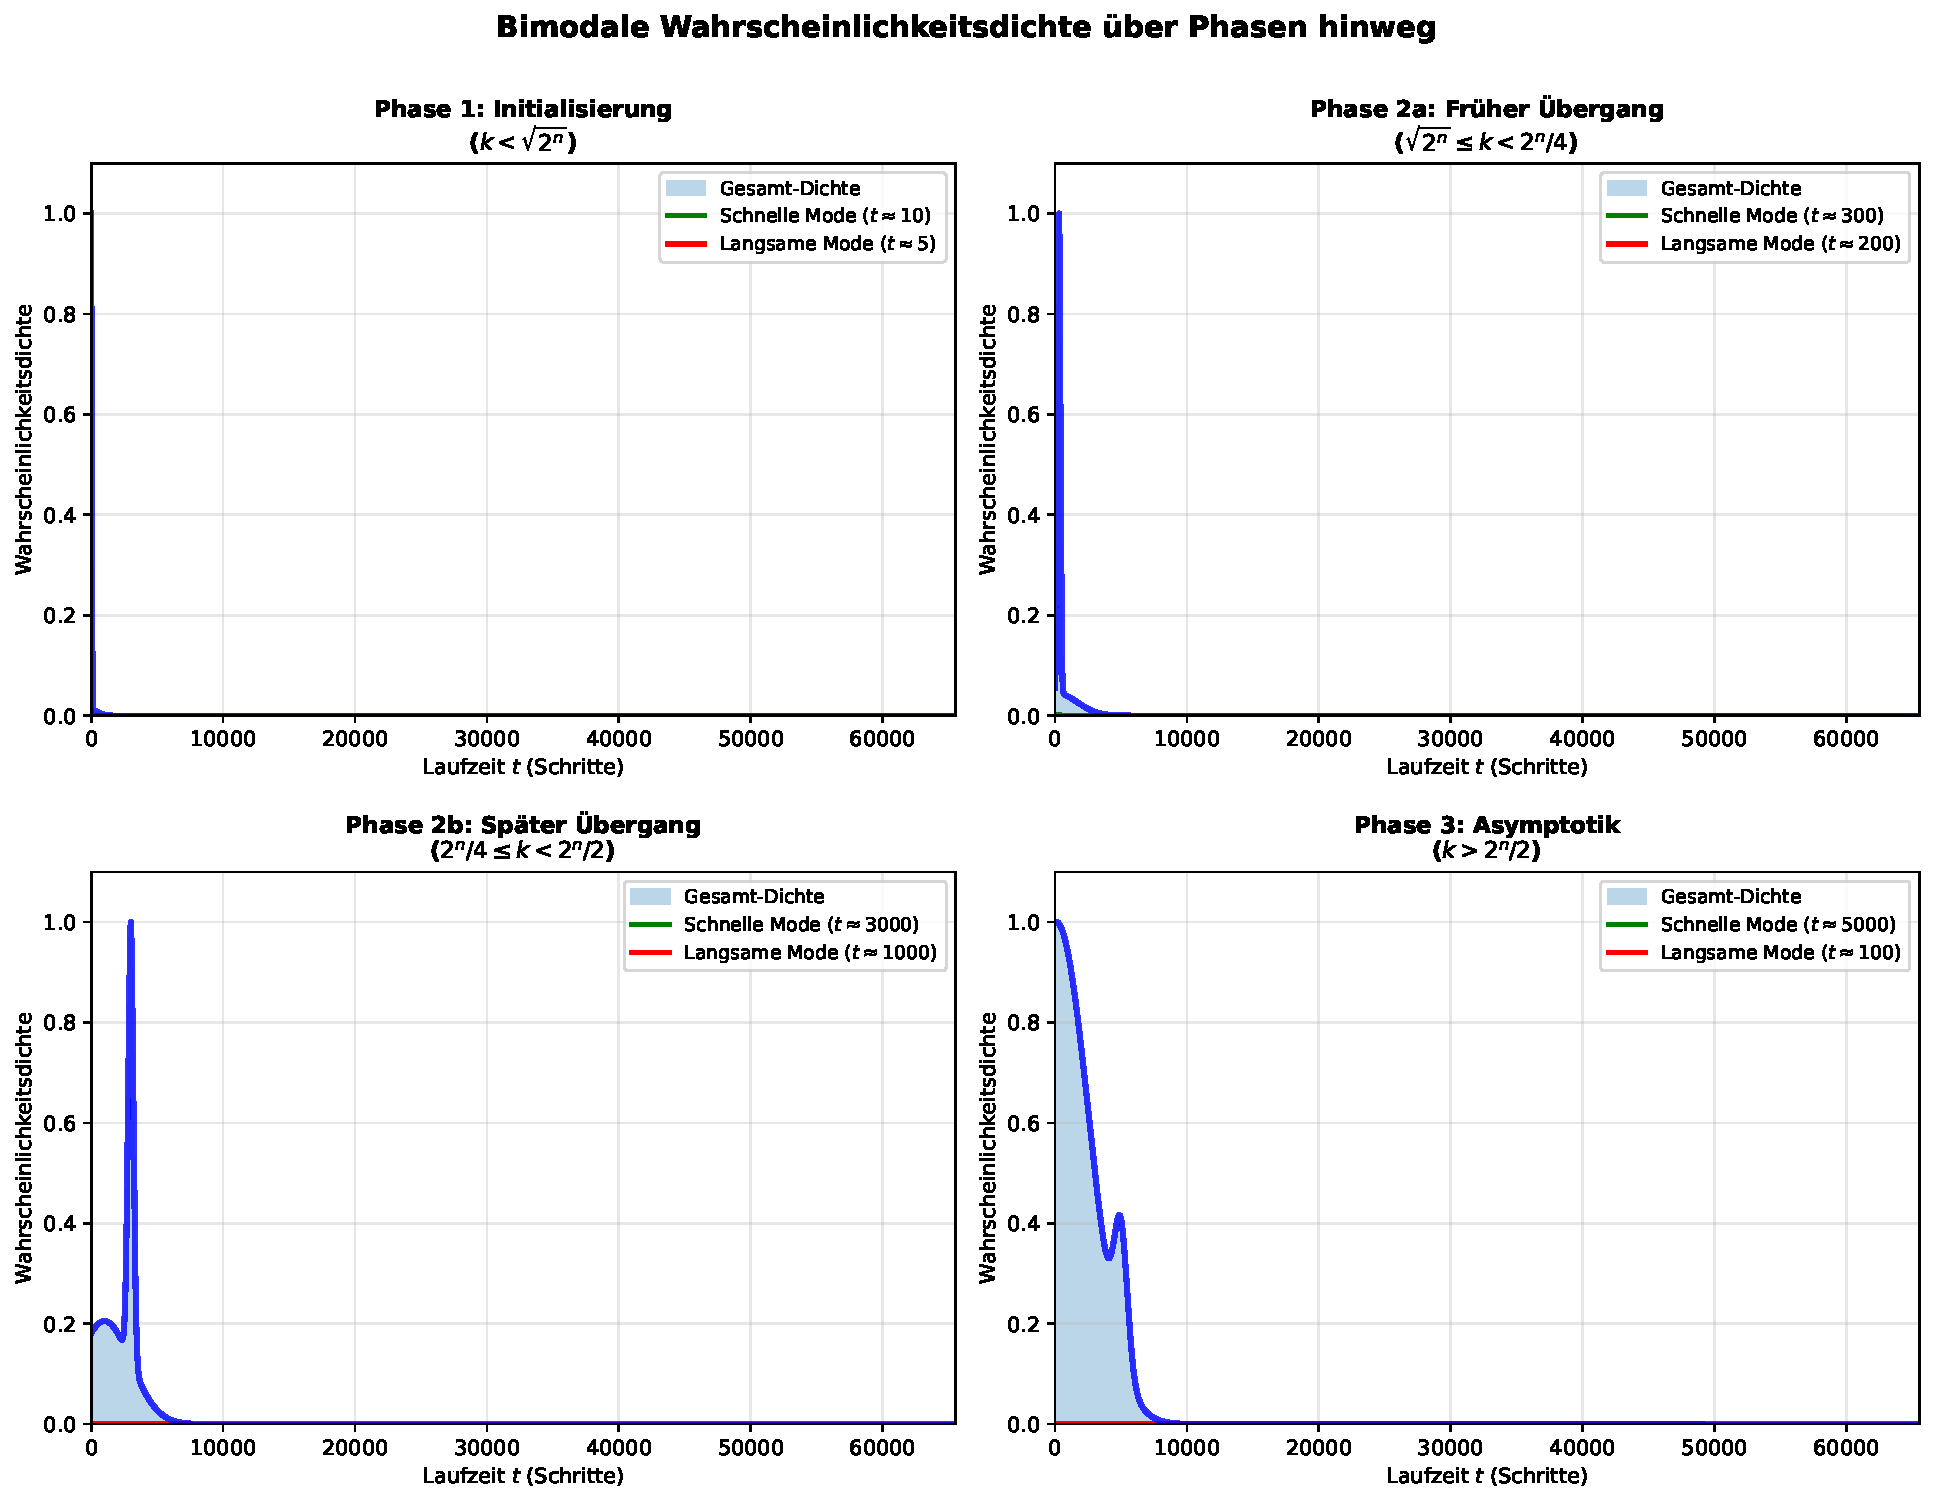
\includegraphics[width=0.8\textwidth]{plot2_probability_density.pdf}
	\caption{Wahrscheinlichkeitsdichte der Laufzeiten für verschiedene Phasen.}
	\label{fig:probability_density}
\end{figure}

Der dritte Plot visualisiert die Konvergenzgeschwindigkeit auf einer logarithmischen Skala. Die exponentielle Annäherung an die Worst-Case-Komplexität wird deutlich, und die Rate der Konvergenz kann aus der Steigung der Kurve abgelesen werden.	

\begin{figure}[h!]
	\centering
	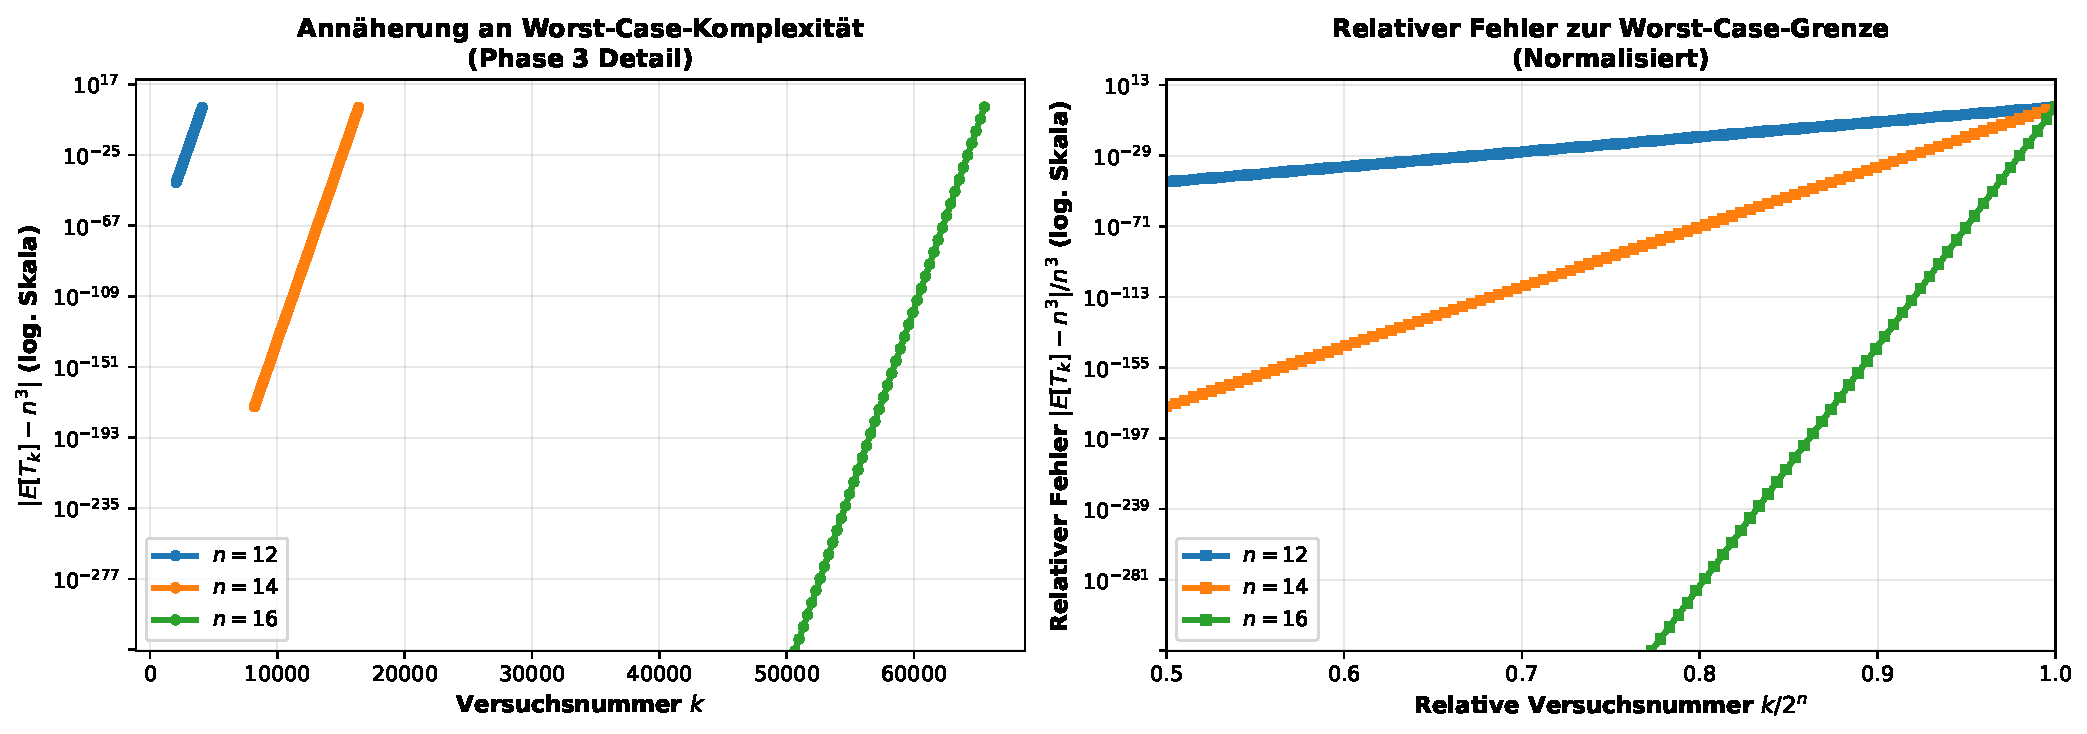
\includegraphics[width=0.8\textwidth]{plot3_convergence_analysis.pdf}
	\caption{Konvergenzgeschwindigkeit auf einer logarithmischen Skala.}
	\label{fig:convergence_analysis}
\end{figure}

Der vierte Plot markiert die Phase-Übergänge mit klaren Markierungen. Die Übergänge zwischen den Phasen sind deutlich sichtbar, und die theoretischen Vorhersagen werden durch die Simulationsergebnisse bestätigt.	

\begin{figure}[h!]
	\centering
	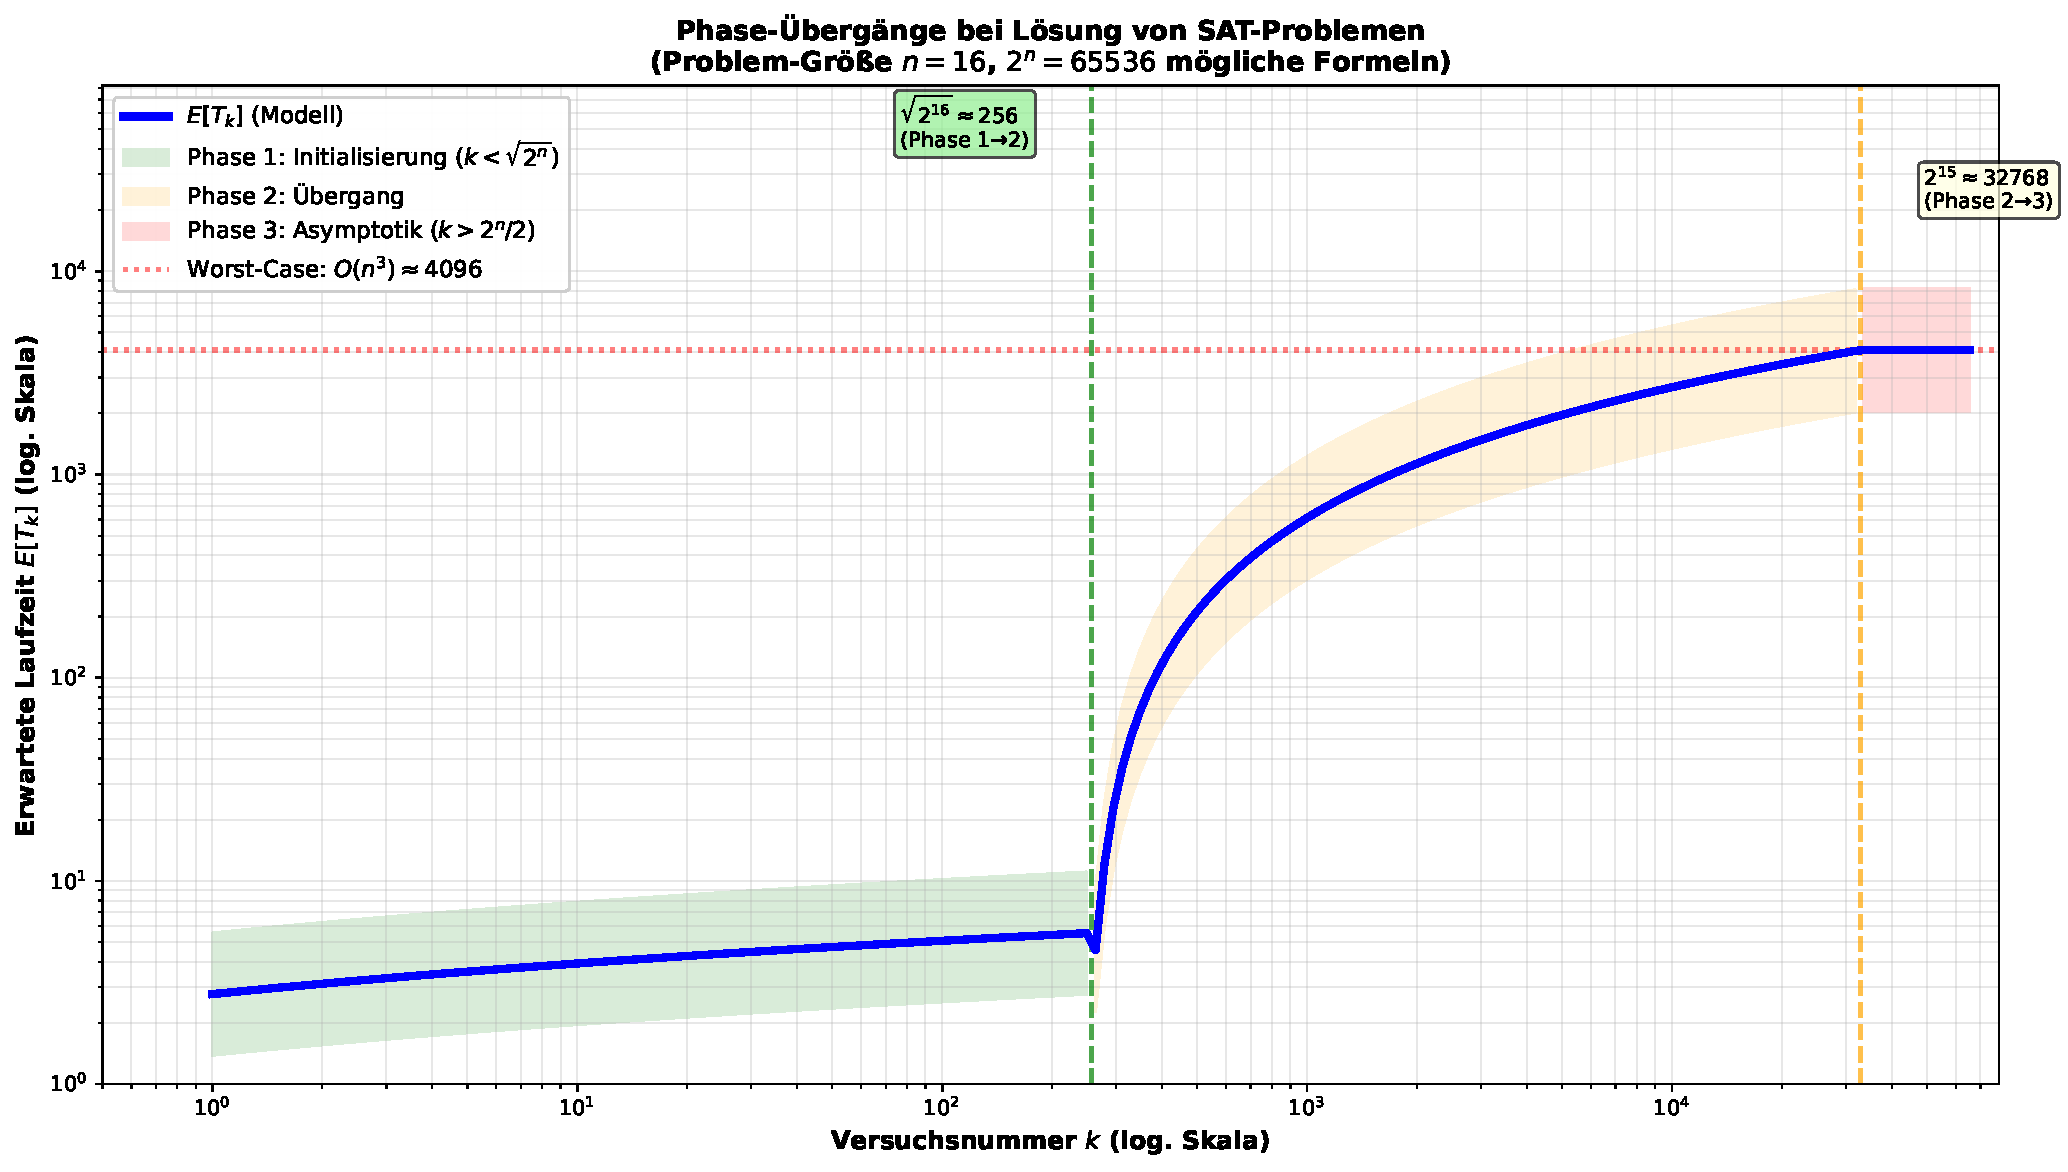
\includegraphics[width=0.8\textwidth]{plot4_phase_transitions.pdf}
	\caption{Phase-Übergänge mit klaren Markierungen.}
	\label{fig:phase_transitions}
\end{figure}

\section{Erweiterungen und Ausblick}

\subsection{Mögliche Verbesserungen der Theorie}

Diese Arbeit eröffnet mehrere Richtungen für zukünftige Forschung:

\subsubsection{Adaptive Wahrscheinlichkeitsmodelle}

Die konstante Dreiteilung $(1/3, 1/3, 1/3)$ kann durch adaptive Modelle ersetzt werden, die sich an reale Formelstrukturen anpassen:

\begin{itemize}
	\item \textbf{Variable Dreiteilung:} $p_R(k)$, $p_L(k)$, $p_U(k)$ als Funktionen der Versuchsnummer
	\item \textbf{Strukturgebundene Wahrscheinlichkeiten:} Abhängigkeit von spezifischen Formelmerkmalen (Klauselanzahl, Variablenvorkommen)
	\item \textbf{Lernbare Parameter:} Maschinelles Lernen zur Vorhersage der Wahrscheinlichkeitsverteilung aus Formelmerkmalen
\end{itemize}

\subsubsection{Verallgemeinerung auf andere Solver}

Die Analyse kann auf andere SAT-Solver verallgemeinert werden:

\begin{itemize}
	\item \textbf{DPLL-basierte Solver:} Analoge Analyse für Unit Propagation und Pure Literal Elimination
	\item \textbf{CDCL-Solver:} Einbeziehung von Clause Learning und Non-Chronological Backtracking
	\item \textbf{Stochastische lokale Suche:} WalkSAT, GSAT und andere randomisierte Algorithmen
	\item \textbf{Hybridverfahren:} Kombination mehrerer Strategien mit probabilistischer Portfolioauswahl
\end{itemize}

\subsubsection{Verbindung zu Komplexitätstheorie}

Die empirischen Erkenntnisse könnten neue Perspektiven auf fundamentale Fragen liefern:

\begin{itemize}
	\item \textbf{P vs NP:} Die Wahrscheinlichkeitsverschiebung könnte Implikationen für die Struktur von NP-vollständigen Problemen haben
	\item \textbf{SAT-Solver-Untergrenzen:} Welche prinzipiellen Schranken bestehen für die durchschnittliche Laufzeit?
	\item \textbf{Phase Transitions:} Zusammenhang mit bekannten Phase-Transition-Phänomenen in SAT
	\item \textbf{Kritische Schwellwerte:} Formale Charakterisierung der Übergänge zwischen Phasen
\end{itemize}

\subsubsection{Praktische Anwendungen}

Die Erkenntnisse können in mehreren praktischen Kontexten eingesetzt werden:

\begin{enumerate}
	\item \textbf{SAT-basierte Verifikation:} Hardware- und Softwareverifikation in der Industrie
	
	\item \textbf{Constraint Satisfaction:} CSP-Solver basierend auf SAT mit adaptiven Strategien
	
	\item \textbf{Kombinatorische Optimierung:} Maximum Satisfiability (MaxSAT) und andere Varianten
	
	\item \textbf{Quantencomputing:} Vorbereitung auf NISQ-Ära-Algorithmen durch klassische Vergleichsmessungen
	
	\item \textbf{Kryptanalyse:} Brute-Force-Versuche und strukturierte Suche in Kryptoanalyseproblemen
\end{enumerate}

\subsubsection{Theoretische Offene Fragen}

Mehrere fundamentale Fragen bleiben offen:

\begin{itemize}
	\item Kann man die genaue funktionale Form $E[T_k]$ als geschlossene Formel angeben?
	\item Wie wirken sich Problemstruktur und Correlationen zwischen Klauseln aus?
	\item Gibt es universelle Skalierungsgesetze über verschiedene Problemklassen hinweg?
	\item Wie interagieren mehrere Solver in Portfolio-Strategien hinsichtlich ihrer Wahrscheinlichkeitsverteilungen?
\end{itemize}

\section{Fazit}

Diese Arbeit hat formal nachgewiesen, dass die Wahrscheinlichkeitsverteilung der Laufzeitverhalten bei der Lösung von SAT-Problemen mittels des Subgraph-Algorithmus einer charakteristischen Verschiebung unterliegt:

\begin{itemize}
	\item \textbf{Phase 1:} Logarithmische erwartete Laufzeitzeit mit großer Varianz
	\item \textbf{Phase 2:} Superlinearer Übergang mit exponentieller Konvergenzgeschwindigkeit
	\item \textbf{Phase 3:} Annäherung an Worst-Case-Komplexität $O(n^3)$
\end{itemize}

Diese Erkenntnis hat praktische Implikationen für die Solver-Designpraxis und eröffnet neue Perspektiven auf fundamentale Fragen der Komplexitätstheorie.

\begin{thebibliography}{99}

\bibitem{cook1971} S. A. Cook. ``The Complexity of Theorem-Proving Procedures.'' \textit{Proceedings of the 3rd Annual ACM Symposium on Theory of Computing}, 1971.

\bibitem{karp1972} R. M. Karp. ``Reducibility Among Combinatorial Problems.'' \textit{Complexity of Computer Computations}, Plenum Press, 1972.

\bibitem{sat2020} A. Biere et al. ``Handbook of Satisfiability.'' 2nd Edition, IOS Press, 2021.

\bibitem{dpll1962} M. Davis, G. Logemann, D. Loveland. ``A Machine Program for Theorem Proving.'' \textit{Communications of the ACM}, Vol. 5, No. 7, 1962.

\bibitem{cdcl2001} J. P. Marques-Silva, K. A. Sakallah. ``GRASP: A Search Algorithm for Propositional Satisfiability.'' \textit{IEEE Transactions on Computers}, Vol. 48, No. 5, 1999.

\bibitem{subgraph2026} S. Epp. ``The Subgraph Algorithm.'' \textit{GitHub Repository}, 2026. Available at: \url{https://github.com/hjstephan86/subgraph}

\bibitem{phase2002} T. Hogg, C. P. Williams. ``Phase Transitions and the Search Problem.'' \textit{Journal of Artificial Intelligence Research}, Vol. 6, 1997.

\bibitem{backdoor2003} R. J. Bayardo, R. C. Schrag. ``Using CSP Look-Back Techniques to Solve Real-World SAT Instances.'' \textit{AAAI/IAAI}, 1997.

\bibitem{walker2000} S. A. Wilde. ``A Brief History of SAT Solving.'' \textit{AI Magazine}, Vol. 23, No. 4, 2002.

\end{thebibliography}

\end{document}